\documentclass[12pt,letterpaper,noanswers]{exam}
%\usepackage{color}
\usepackage[usenames,dvipsnames,svgnames,table]{xcolor}
\usepackage[margin=0.9in]{geometry}
\renewcommand{\familydefault}{\sfdefault}
\usepackage{multicol}
\pagestyle{head}
\usepackage{hyperref}
\usepackage[numbered,autolinebreaks,useliterate]{mcode}
\newcommand{\mb}[1]{\underline{#1}}

\header{AM 22b Problem Set 09}{}{Due Thurs Apr 22 at 6pm EDT}
\runningheadrule
\headrule
\usepackage{diagbox}
\usepackage{graphicx} % more modern
%\usepackage{subfigure} 
\usepackage{amsmath} 
\usepackage{amssymb} 
%\usepackage{gensymb} 
%\usepackage{natbib}
\usepackage{hyperref}
%\usepackage{enumitem}
%\setlength{\parindent}{0pt}
%\usepackage{setspace}
%\pagestyle{empty}  
%\newcommand{\Sc}[0]{
%{\color{BlueViolet}\S}
%}
\usepackage{tcolorbox}

\begin{document}
 \pdfpageheight 11in 
  \pdfpagewidth 8.5in
  
% divergence, divergence theorem, intro to diff eq, linear superposition of solutions of diff eq., basic separation of variables method.

\begin{questions}
\question Log in to WeBWorK and complete the problems assigned there under pset09.

\question 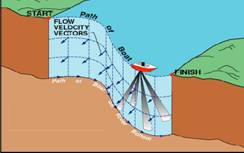
\includegraphics{img/S20pset08USGS.png}

Refer back to problem set 08 for the formula that was derived to compute the flux of the water given boat velocity and water velocity information.

\begin{parts}
\item We have velocity measurements for the water flow in a single vertical column of a river.  For this column, the boat is moving $0.318$ ft/s east and $-0.205$ ft/s north for a time period of $\Delta t = 0.56$ s.  The column is made up of multiple boxes, and each of the boxes has a depth of $0.2$ ft.  Find an approximation of the area of one of the boxes in this column.
\item Open AM22bPSet09.m to access velocity data at thirteen different depths in the water column.  Use the boat velocity and time information from part (a) along with this flow data to find an approximation of the flux of water downstream through the column.  Provide a written explanation of how you used the data to approximate the flux, and include a screenshot of your calculation code, along with your estimated value, in your Gradescope submission.
\end{parts}



\question Consider the second order differential equation $a\frac{d^2y}{dt^2} + b\frac{dy}{dt} + cy = 0$ where $a,b,c$ are constants.  Let $y_1(t) = e^{-2t}\cos 5t$ and $y_2(t) = e^{-2t}\sin 5t$.
\begin{parts}
\item Is the differential equation linear or nonlinear?  How do you know?
\item Find $a,b,c$ such that $y_1(t)$ and $y_2(t)$ are both solutions to the differential equation.
\item Consider a function, $y_3(t)$, that is a linear combination of the two solutions.  Let $y_3(t) = k_1 y_1(t) + k_2 y_2(t)$.  Either show that $y_3(t)$ is a solution to the differential equation, or show that it is not.
\end{parts} 





% \question Let $W$ be the solid region bounded below by $z = x^2+y^2$ and bounded above by $z = \sqrt{6-x^2-y^2}$.  Let $S_1$ be the paraboloid forming the lower surface of $W$, oriented upward.  Let $S_2$ be the spherical cap forming the upper surface of $W$, also oriented upward.

% \begin{parts}
% \item \emph{On PSet 08 you found the flux of $\underline F = \langle x, y, z\rangle$ upward through $S_1$.}

%  Use the divergence theorem to find the flux of $\underline F = \langle x, y, z\rangle$ outward through $\partial W$, the boundary of $W$.

%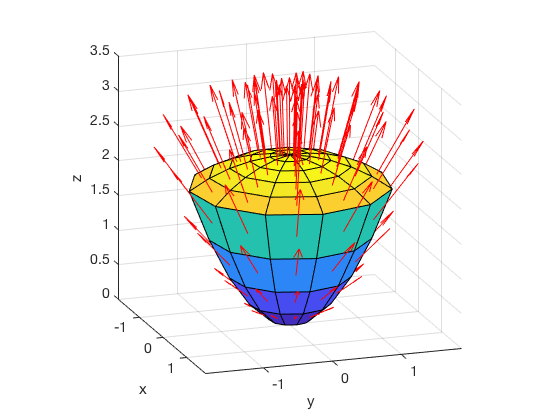
\includegraphics[width=0.4\linewidth]{img/pset11p4-18.png}


% \item Determine (without integration) the flux through $S_2$, with upwards orientation.

% \end{parts}

\question 
\begin{parts}
\item Let $W$ be a solid region of volume $V$ surrounded by a closed surface $S$, oriented outward.  Show that $\displaystyle \frac{1}{3}\int_S \vec r\cdot d\vec A = V$.  Here the vector field is $\vec r = x\vec i + y\vec j + z\vec k$.  

\emph{This is a remarkable result: it creates a way to approximate the volume of a region when you only have information about points on the surface of the region.}
\begin{solution}
For this vector field, $\text{div }\vec F = 1 + 1 + 1 = 3$, so we have \[\frac{1}{3}\int_S\vec r\cdot d\vec A = \frac{1}{3}\int_W 3\ dV = \int_W \ dV = V.\]
\end{solution}
\item Suppose $\text{div }\underline F = x^2+y^2+3$.  Find a surface, $S$ such that $\int_S\underline F\cdot d\underline A$ is negative (for any vector field where $\text{div }\underline F = x^2+y^2+3$), or explain why no such surface exists.
\begin{solution}
By the divergence theorem,
\[\int_{\partial W} \vec F \cdot d\vec A = \int_W \text{div }\vec F\ dV = \int_W (x^2+y^2+3)\ dV,\] so the flux outward through a closed surface will always be positive.  Let $S$ be a closed surface oriented inward.  Now the flux through the surface will be negative (since the flux will be the negative of the flux outward through that surface).
\end{solution}
\end{parts}

\question 
%\begin{parts}
Let $S$ be the portion of the unit sphere centered at the origin that is above the cone $z = \sqrt{x^2+y^2}$.  \emph{Note that the term 'sphere' refers to a surface, not a solid}.  Let $\displaystyle\underline F = \langle xy+\cos z, -yx+x^2+z^3,2z^2+x\rangle$.  Find $\displaystyle\int_S\underline F\cdot d\underline S$.

\emph{Radial symmetry in this problem can help you simplify the integrals.  If you use cylindrical or spherical, integrate first with respect to $\theta$, so that cancellations due to radial symmetry happen before you tackle the rest of the integral.}
%\part Find the area of the portion of the unit sphere (the sphere of radius $1$ and centered at the origin) that is inside the cylinder $\displaystyle x^2+y^2 = \frac{1}{2}$ and $z>0$.  The area of a surface is given by $\displaystyle\int_S dS = \int_S \left\Vert d\underline S\right\Vert$.

%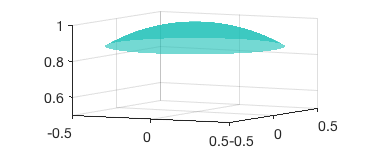
\includegraphics[width=2in]{img/Math212p2q1-18.png}
%\end{parts}

% \question A vector field is spherically symmetric about the origin if, on every sphere centered around the origin, the vector field has a constant magnitude and either points away from the origin (in the direction of $\mb r$) or towards the origin (in the direction of $-\mb r$).

% A vector field that is spherically symmetric can be written in terms of the spherical coordinate $\rho = \Vert \mb r \Vert$ and a unit vector pointing away from the origin, $\mb e_{\rho} = \mb r/\Vert \mb r \Vert$.  To be well-defined at the origin, the vector field must be zero there.

% We write $\mb F = f(\rho)\mb e_{\rho}$, with $f(0) = 0$.

% \begin{parts}
% \part Show that $\nabla \cdot \mb F = \dfrac{1}{\rho^2}\dfrac{d}{d\rho}\left(\rho^2 f(\rho) \right)$, $\rho \neq 0$.  \emph{Compute the divergence in Cartesian coordinates and then change coordinate systems.  Note that $f_x(\rho) = f_{\rho}(\rho)\frac{\partial\rho}{\partial x}$.}
% \begin{solution}
% Q6a: We have $$\underline F = f(\rho) \underline e_{\rho} = (f(\rho)/\rho)\langle x, y,z\rangle$$.
% $$\nabla \cdot \underline F = \partial_x (f(\rho)x/\rho) + \partial_y (f(\rho)y/\rho) + \partial_z (f(\rho)z/\rho)$$.  Using the product rule on each term,
% $$\Rightarrow \nabla \cdot \underline F = 3f(\rho)/\rho + x\partial_x (f(\rho)/\rho) + y\partial_y (f(\rho)/\rho) + z\partial_z (f(\rho)/\rho)$$.  Using the chain rule,
% $$\Rightarrow \nabla \cdot \underline F = 3f(\rho)/\rho + xd_{\rho} (f(\rho)/\rho)\rho_x + yd_{\rho} (f(\rho)/\rho)\rho_y + zd_{\rho} (f(\rho)/\rho)\rho_z$$.
% We have $$\rho = (x^2+y^2+z^2)^{1/2}$$ so $$\rho_x = x/\rho$$, etc.  Substituting and combining terms, we now have
% $$ \nabla \cdot \underline F = 3f(\rho)/\rho + \frac{x^2+y^2+z^2}{\rho}d_{\rho} (f(\rho)/\rho)$$.
% $$\Rightarrow \nabla \cdot \underline F = 3f(\rho)/\rho + \rho d_{\rho} (f(\rho)/\rho)$$.  Expanding via the product rule, this is
% $$\nabla \cdot \underline F = 3f(\rho)/\rho + \rho (f'/\rho - f/\rho^2) = 2f/\rho + f'$$.  Now we rearrange to move this towards the form we were given:
% $$\nabla \cdot \underline F = \frac{1}{\rho^2}(2\rho f + \rho^2 f') = \frac{1}{\rho^2}\frac{d}{d\rho}(\rho^2 f) $$.

% There are other ways to do this algebra.
% \end{solution}
% \part Show that for $\mb F$ spherically symmetric, if $\nabla \cdot \mb F = 0$ away from the origin then $\mb F = k\dfrac{1}{\rho^2}\mb e_{\rho}$, $\rho\neq 0$, for some constant $k$.  \emph{Argue that $\rho^2f(\rho)$ is a constant.}
% \begin{solution}
% Assume $\nabla\cdot\underline F = 0$ (away from $\rho = 0$), so $\frac{1}{\rho^2}\frac{d}{d\rho}(\rho^2f(\rho)) = 0$.  $\Rightarrow \frac{d}{d\rho}(\rho^2f(\rho)) = 0$ so $\rho^2f(\rho) = k$ for some constant $k$, and we find that $f(\rho) = k\frac{1}{\rho^2}$.  $\underline F = f(\rho)\underline e_{\rho}$ so $\underline F = k\frac{1}{\rho^2}\underline e_{\rho}.$

% \end{solution}
% \part For an electric field $\mb E$, a form of \textbf{Gauss's Law} states that $\nabla\cdot E(\mb r)$ is equal to the charge density at every point.  Find $\mb E$ when $\displaystyle\nabla\cdot \mb E = \left\{\begin{array}{c}\delta_0\quad \Vert \mb r\Vert \leq a \\ 0\quad \Vert \mb r\Vert > a\end{array}\right.$ for some non-negative $a$.

% Assume that $\mb E$ is spherically symmetric and is continuous everywhere. 

% \emph{When you integrate with respect to $\rho$, a constant of integration will arise.  You integrate two different functions, producing two different constants.  Use the definition of `spherically symmetric' to set one of the constants.  Use continuity at $\rho = a$ to set the other constant.}
% \begin{solution}
% $\underline E$ is spherically symmetric, so $\underline E = f(\rho)\underline e_{\rho}$ away from the origin, and at the origin, $\underline E = \underline 0$.

% We have $\nabla \cdot \underline E = 0$ when $\rho > a$, so $\underline E = k\frac{1}{\rho^2}\underline e_{\rho}$ for $\rho > a$.

% We have $\nabla \cdot \underline E = \delta_0$ when $\rho < a$, so $\frac{1}{\rho^2}\frac{d}{d\rho}(\rho^2f(\rho)) = \delta_0$.  This implies $\frac{d}{d\rho}(\rho^2f(\rho)) = \delta_0\rho^2$ so $\rho^2f(\rho) = \frac{\delta_0}{3}\rho^3 + c$.  Rearranging, we have $f(\rho) = \frac{\delta_0}{3}\rho + c\rho^{-2}$.  $f(0) = 0$ so $c = 0$ is necessary.

% For $\rho < a$ we have $\underline E = \frac{\delta_0}{3}\rho \underline e_{\rho}$.  For $\rho = a$ this would be $f(a) = \frac{\delta_0}{3}a$.

% For $\rho > a$ we have $\underline E = k\frac{1}{\rho^2}\underline e_{\rho}$.  For $\rho = a$ this would be $f(a) = k/a^2$.

% For continuity at $r = a$ we need $\frac{\delta_0}{3}a = k/a^2$ so $k = \frac{\delta_0}{3}a^3$.
% \end{solution}

% \end{parts}


% \question Let $P$ be the prism bounded below by the plane with equation $z = 0$, on the sides by planes with equations $y = 0, y = 5, x = 0$ and above by the plane with equation $z = 2-x$.
% \begin{parts}
% \item Sketch $P$.
% \item Set up an integral for the volume of $P$.  \emph{Do not integrate}.
% \item Let $S' = \partial P$.  Let $S$ be the surface obtained by removing the bottom face (the face in the $xy$-plane) from $S'$, with $S$ inheriting its orientation from $S'$.  Compute the flux across $S$ of the vector field $\underline F = \langle x^3y, x^2y^2, x^2y(z+1)\rangle$.
% \end{parts}

\question Consider the initial value problem $\frac{dy}{dt} = \sqrt{y}$, $y(0) = 1$.  
\begin{parts}
\part Working in matlab, use Euler's method to compute three different approximate solutions.  Use $\Delta t = 1.0, 0.5, 0.25$ over the interval $0\leq t\leq 4$.  Provide your approximations for $y(2)$ and $y(4)$ for each method.
\item Graph your three solutions (all on the same axes, so that they can easily be compared).
\item Make a prediction about $y(2)$ and $y(4)$ for the actual solution to the initial value problem.
\item Improve your approximation: choose a small enough step size, $h = \Delta t$, so that your approximation for $y(4)$ using $h$ and using $h/2$ differ by less than $0.5$\%.
\end{parts}

\begin{lstlisting}
% sample code for Euler's method
clear('tval','yval')
tval(1) = 1790; % initial time
yval(1) = 3929214; % initial population
k = 1; % index
dt = 2; % time step
const = 0.0223;
endtime = 2050;
while tval(k) < endtime
    dydt(k) = yval(k)*const; % dP/dt = const * P
    tval(k+1) = tval(k) + dt;
    yval(k+1) = yval(k) + dydt(k)*dt; % Pnew approx= Pold + dP/dt*delt t
    k = k+1;
end
plot(tval,yval)
\end{lstlisting}



\end{questions}

\end{document}
